\documentclass{article}
% s e l e c c i o n a e l t i p o de documento
\usepackage[spanish]{babel}
%
\usepackage[T1]{fontenc}
\usepackage[latin1]{inputenc}
\usepackage{graphicx}
\usepackage{amsmath}
\begin{document}
% i n i c i o d e l cuerpo d e l documento
\title{Laboratorio 6: Manipulaci\' on de imagenes con punteros}
\author{Jean Carlos Chavarr\' ia Hughes B11814}
\maketitle
% t i t u l o d e l documento
\begin{abstract}
Laboratorio 6 de el curso IE 0217.
\end{abstract}
\section{Introducci\' on}
Este documento corresponde al reporte de sexto laboratorio del curso IE0217, en el cual se trabaj\' o con distintos funciones de la librer\' ia OpenCV, para la cual se implementaron varias funciones que trabajaran con imagenes, las modificaran, filtros y otras cosas.

Cabe destacar que los archivos de c\' odigo fuente difieren un poco de la plantilla suministrada por el asistente, esto \' unicamente con el fin de simplificar y personalizar la clase, pero es completamente equivalente.

\begin{figure}[hbtp]
\caption{OpenCV Library}
\centering

\includegraphics[scale=1]{imagenes/OpenCV_Logo_with_text.png}
\end{figure}


\section{ImagenRGB}
\subsection{Imread()}
La primer parte del laboratorio consisti\' o en utilizar la funci\' on \textbf{imread()} de la libreria, la cual se escarga de almacenar una imagen en un objeto tipo \textbf{Mat}. Los objetos tipo Mat son parte de una clase que se encuentra en la librer\' ia y la cual tiene caracter\' isticas muy interesantes para el manejo de la informaci\' on de una imagen. B\' asicamente cuenta con dos miembros importantes que definen las dimensiones del objeto, y un puntero llamado data, que se encarga de apuntar la posici\' on de memoria donde esta la informaci\' on de la imagen. 
Se puede observar el fichero \textbf{imagenRGB.cpp} donde se encuentran los constructores dise\~ nados para llevar a cabo esta parte del laboratorio al igual que el destructor.

\subsection{M\' etodo showImage()}
Tal y como se solicita en el enunciado, para realizar esta funci\' on, se utiliz\' o la funci\' on de la libreria llamada \textbf{imshow()}, seguida de la funci\' on \textbf{waitKey(0)}. La parte de la funci\' on donde se asigna un puntero a imagen.data es precisamente donde se esta asignando el valor de la matriz de la imagen al arreglo correspondiente.
\begin{verbatim}
void ImageRGB::showImage(void){
	Mat imagen(this->height, this->width,CV_8UC3);
	imagen.data = this -> data;
	imshow("Ventana1",imagen);
	waitKey(0);
	cout<<"showImage() executed"<<endl;
	}
\end{verbatim}

\subsection{Pasar a escala de grises}
Para realizar la modificaci\' on de la imagen a color a escala de grises, se tuvo que investigar un poco m\' as sobre el tipo de canales utilzados y la cantidad de bits por canal. Luego, se sigui\' on con el procesimiento en tanto que se utiliz\' o la conversi\' on \textbf{luma} para realizar la transformaci\' on. Finalmente el m\' etodo se encarga de guardar la imagen en el directorio como \textbf{imagen gray scale.png}.
Fue necesario crear cuatro matrices, una para que almacenara cada canal y otra para que almacenara el resultado de la suma de la ecuaci\' on \textbf{luma}.

\begin{verbatim}
void ImageRGB::toGray(void){
	Mat imagen(this->height, this -> width, CV_8UC3);
	imagen.data = this -> data;
	cout<<"passing to gray scale"<<endl;
	
	float* B= new float[(this->height)*(this->width)];//matriz de azul
	float* G= new float[(this->height)*(this->width)];//matriz de verde
	float* R= new float[(this->height)*(this->width)];//matriz de rojo
	float* Y= new float[(this->height)*(this->width)];//matriz final

	int altura = this->height;
	int anchura = this->width;

	for(int i = 0; i<(altura*anchura); i=i+3){
		B[i]=(float)this->data[3*i];
		G[i]=(float)this->data[3*i+1];
		R[i]=(float)this->data[3*i+2];
		Y[i]=0.299*R[i]+0.587*G[i]+0.114*B[i];
	}

	Mat imagenGray(altura, anchura,CV_32FC1);//Float,, C channel, 1 un canal
	cout<<"passing to gray scale"<<endl;
	//imshow("escala grises",imagenGray);
	imwrite("imagen_gray_scale.png",imagenGray);
	
}
\end{verbatim}

\subsection{drawCircle()}.
Finalmente para esta funci\' on, se implement\' o la funci\' on de la libreria \textbf{circle()}, la cual cabe destacar que recibe como par\' ametros, la posici\' on del centro del c\' irculo a dise\~ nar y el radio correspondiente.
Finalemente la imagen se almancena en un nuevo fichero llamado \textbf{imagen con circulo.png}.

\begin{verbatim}
void ImageRGB::drawCircle(int x, int y, unsigned int radius){
	Mat imagen(this -> height,this -> width,CV_8UC3);
	imagen.data = this -> data;
	if ( x<width && y<height && (width-y)>radius && (height-x)>radius)
	{
		circle(imagen,Point(x,y),radius,Scalar(255,0,0,0),-1);
		cout<<"drawing a circle"<<endl;
		imwrite("imagen_con_circulo.png",imagen);
	}
	else
	{
		cout<<"Out of bounding"<<endl;
	}
	}
\end{verbatim}

\section{ImagenGS}
Adem\' as de los m\' etodos descritos en las secciones anteriores, se definen nuevos m\' etodos para esta clase.

\subsection{medianFilter()}
Este m\' etodo recibe un par\' ametro entero que es la medida n para el kernel del filtro, recordando que es una matriz cuadrada, pero debe ser impar y mayor que 1. 
B\' asicamente el m\' etodo se encarga de remover el ruido de una imagen, lo cual genera una nueva imagen pero un poco difundida en el fichero: \textsc{imagen median filter.png}. Por ejemplo una imagen como la que aparece en la Figura \ref{fig:original}, puede ser vista como la que aparece en la Figura \ref{fig:medianFilter}.

\begin{verbatim}
void ImageGS::medianFilter(int size){
	Mat imagen(this->height, this -> width, CV_8UC3);
	imagen.data = this -> data;
	cout<<"Aplicando el filtro medio"<<endl;
	
	int altura = this->height;
	int anchura = this->width;
	
	for(int i = (3*(size+size*anchura)); i < (3*((anchura*altura)-(size+size*anchura))); i++){//Posiciones de la matriz Y que se deben recorrer
		int sumatoriaTotal = 0;
		for(int j = -size; j <= size; j++){//la variable j determina el ancho de kernel
			for(int g = -size; g <= size; g++){//la variable i determina el alto del kernel
				
				sumatoriaTotal = sumatoriaTotal + (int)this->data[i + 3*j + 3*g*anchura];
				
			}	
		}
		
		sumatoriaTotal = sumatoriaTotal/((2*size+1)*(2*size+1));//se pasa la parte entera
		imagen.data[i] = sumatoriaTotal;		
	}
	
	Mat imagenFilter(altura, anchura,CV_8UC3, imagen.data);//Float,, C channel, 1 un canal
	imwrite("imagen_median_filter.png",imagen);
	//imshow("Median Filter",imagen);
	waitKey(1950);
}
\end{verbatim}


\begin{figure}[hbtp]
\caption{Imagen con el filtro medio aplicado.}
\centering
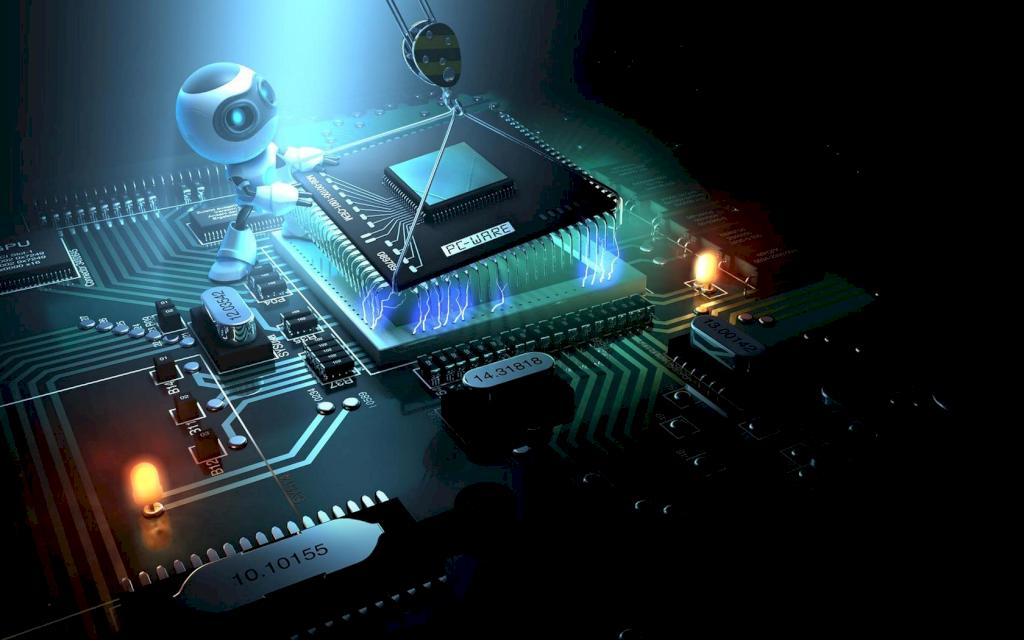
\includegraphics[scale=0.5]{imagenes/imagen1.png}
\label{fig:original}
\end{figure}

\begin{figure}[hbtp]
\caption{Imagen con el filtro medio aplicado.}
\centering
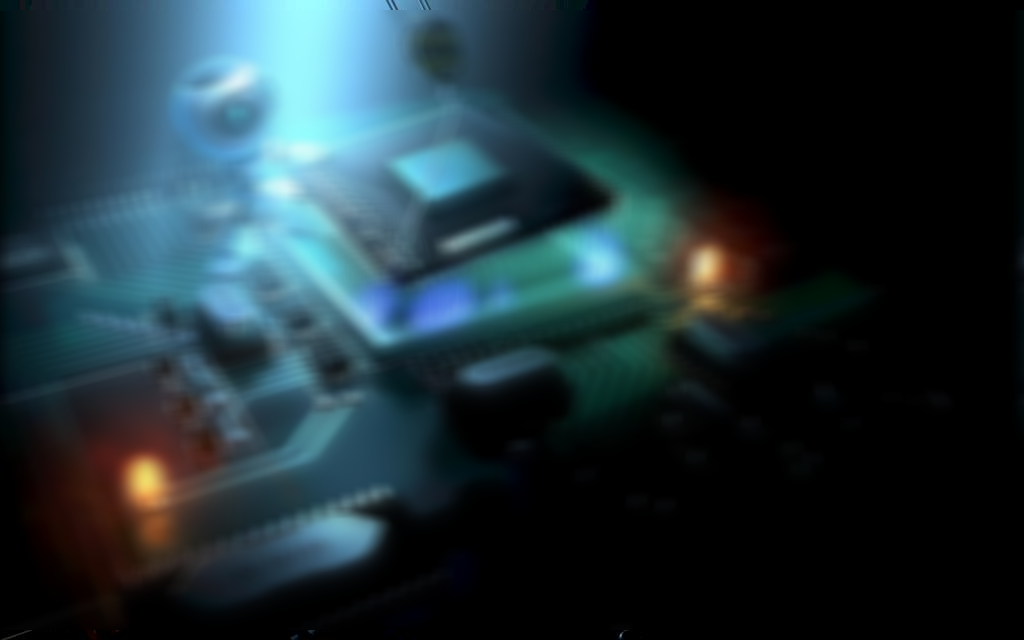
\includegraphics[scale=0.5]{imagenes/imagen_median_filter.png}
\label{fig:medianFilter}
\end{figure}


\subsection{sobelOperator()}
El operador sobel se encarga de crear una nueva image epro en la cual solo se esten presentes los bordes, o ejes de la imagen original. Por ejemplo se puede pensar en una imagen que tenga ecuaciones matem\' aticas, integrales, etc. Pero esta un poco borrosa, entonces despu\' es de aplicad este m\' etodo, solo van a aparecer las ecuaciones m\' as f\' acil de observar pues se tomaran los bordea de cada elemento. Funciona tanto para imagenes a color como imagenes en escala de grises y se basa en la comvoluci\' on de un par de matrices o kernels predefinidos como:

\begin{align}
Gx:
 \left( \begin{array}{ccc}
-1 & 0 & +1 \\
-2 & 0 & +2 \\
-1 & 0 & +1 \end{array} \right)
\end{align}

\begin{align}
Gx:
 \left( \begin{array}{ccc}
+1 & +2 & +1 \\
0 & 0 & 0 \\
-1 & -2 & -1 \end{array} \right)
\end{align}



\subsection{threshold()}
El m\' etodo del umbral, o el \textbf{thresholding} b\' asicamente se encarga de generar imagenes binarias siguiendo m\' etodos basados en la forma de los histogramas de cada imagen (existen otros m\'
 etodos pero se eligi\' o este por simplicidad).
 
 Por ejemplo se puede observar la misma imagen de la Figura \ref{fig:original} con el filtro aplicado, que se obtiene la imagen de la Figura \ref{fig:umbral}.
 
 \begin{figure}[hbtp]
 \caption{Imagen con el m\' etodo threshold aplicado.}
 \centering
 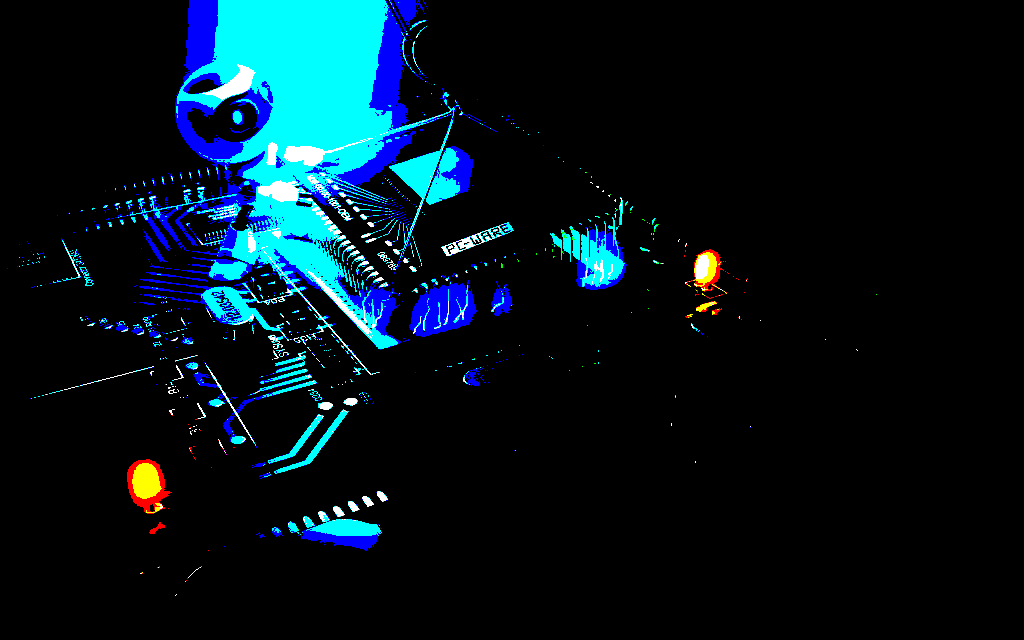
\includegraphics[scale=0.5]{imagenes/imagen_otsu_threshold.png}
 \label{fig:umbral}.
 \end{figure}
 

\subsection{variance}
Finalmente el m\' etodo de varianza se encarga de procesar la imagen para encontrar la varianza probal\' istica dentro de un vecindario de tama\~ no k con la f\' ormula motrada en la ecuaci\' on (1) de la gu\' ia de laboratorio.

Tal como describe Vijay Kumar y Priyanka Gupta en el art\' iculo \textbf{Importance of statical peasures in digital image processing}, la varianza es una medidad de que tan lejos un conjunto de valores se esparcen, en tanto que se puede entender como uno de los momentos de distribuci\' on de imagenes.

\end{document}
